\section{Database-modellering}\label{databasemodellering}

I projektet gør vi brug af en database, som er udleveret fra UCL. Den er struktureret i Microsoft SQL Server Management Studio, som bruger sproget Structured Query Language(SQL).



Vi har valgt at gøre brug af en database til vores projekt både for at lære at bruge SQL, men også for at håndtere data, som skal bruges senere uden, at det mistes når programmet slukkes, og skal kunne tilgåes på andre maskiner end den, der har indsat dataen.

\begin{figure}[H]
    \makebox[\textwidth][c]{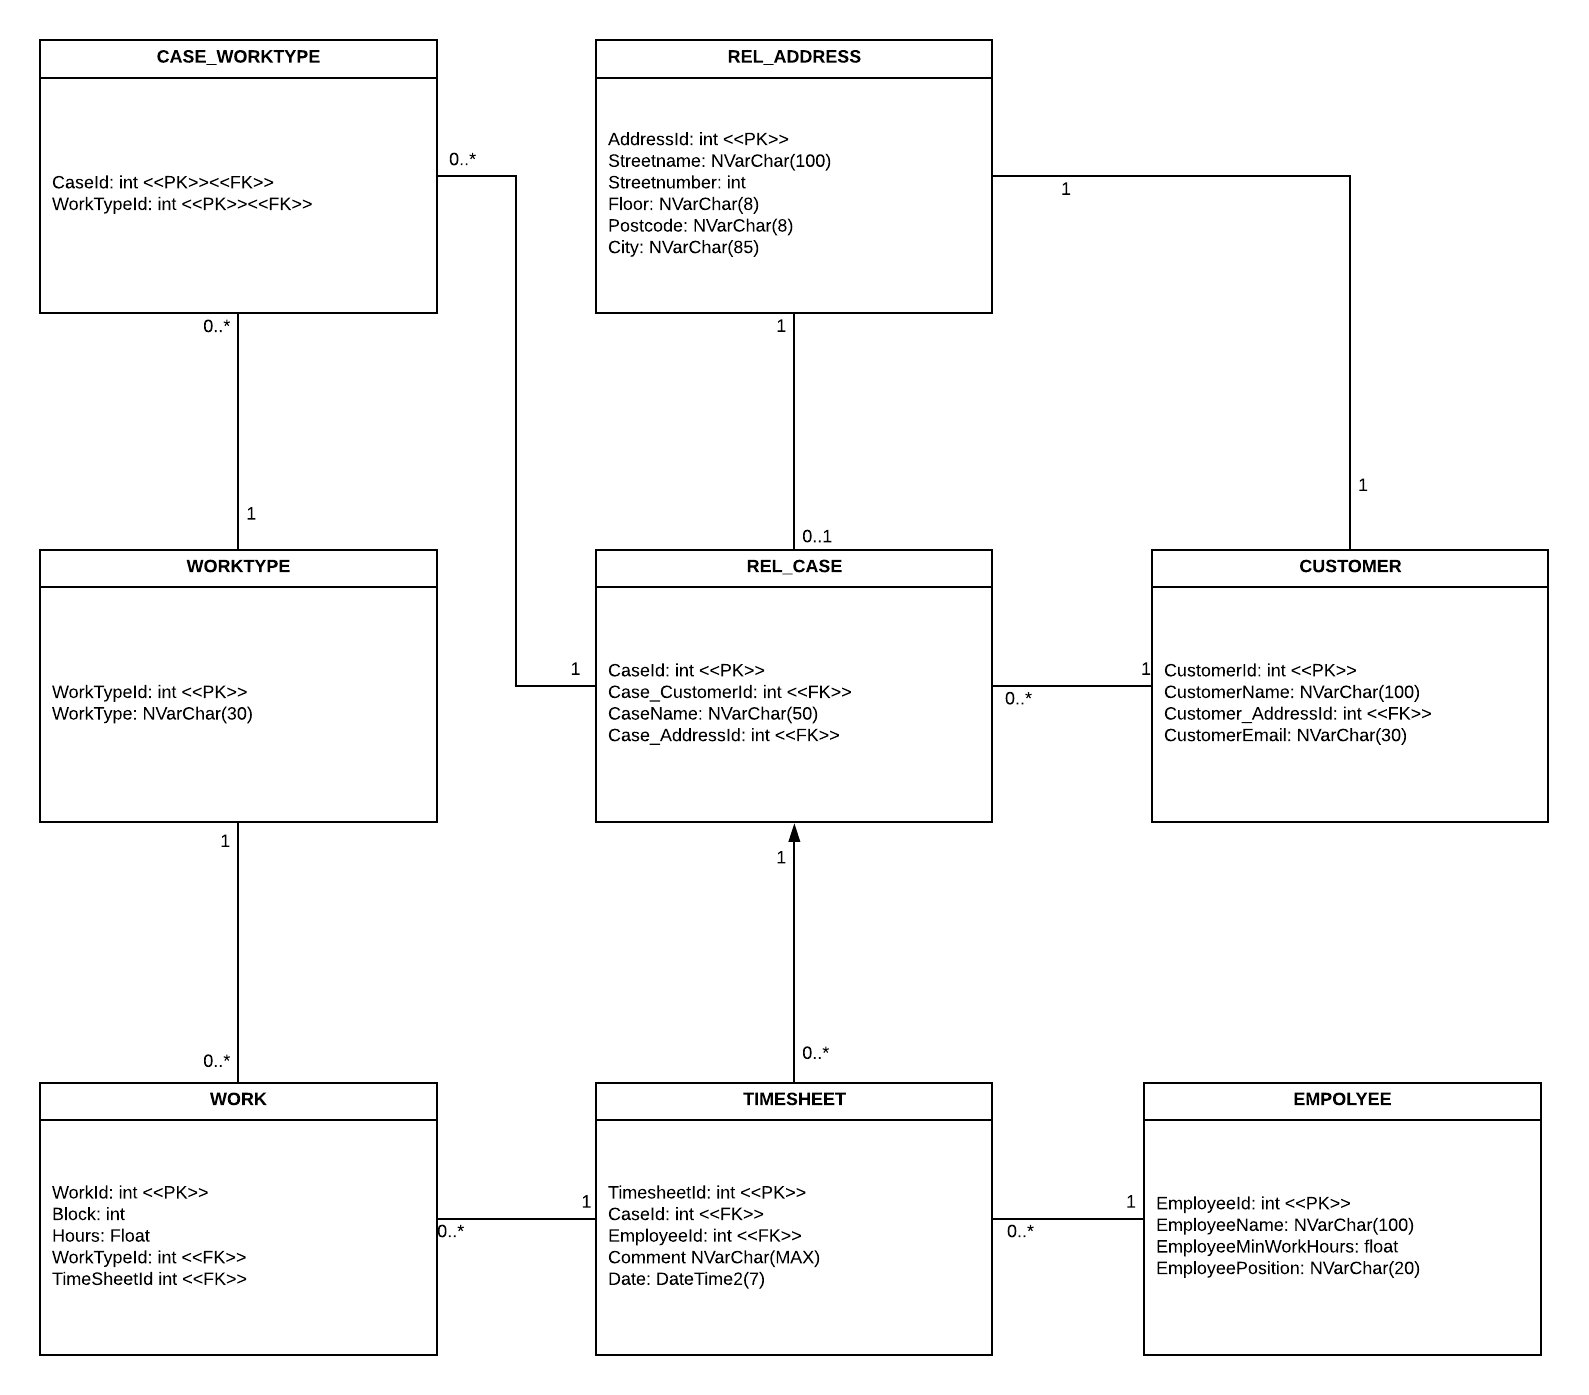
\includegraphics[scale = .8]{Database.png}}
    \caption{Her vises UML database diagrammet over den implementeret database}
    \label{fig:DatabaseDiagram}
\end{figure}

I figur \ref{fig:DatabaseDiagram} ses et oversigt over databasen for HHS.
Der er lavet otte tabeller, som alle overholder den tredje normaliserings form. \cite{Database}
Dette kan for eksempel ses ved, at vi havde en mange til mange relation mellem WORKTYPE og REL\_CASE og derfor var vi nød til at lave et ekstra table, som kom til at hede CASE\_WORKTYPE, der sørger at dette ikke at tilfældet, da der derved skabes en en til mange relation fra WORKTYPE og CASE\_WORKTYPE og fra REL\_CASE til CASE\_WORKTYPE.

\subsection{Database procedurer}

\begin{figure}[h]
    \makebox[\textwidth][c]{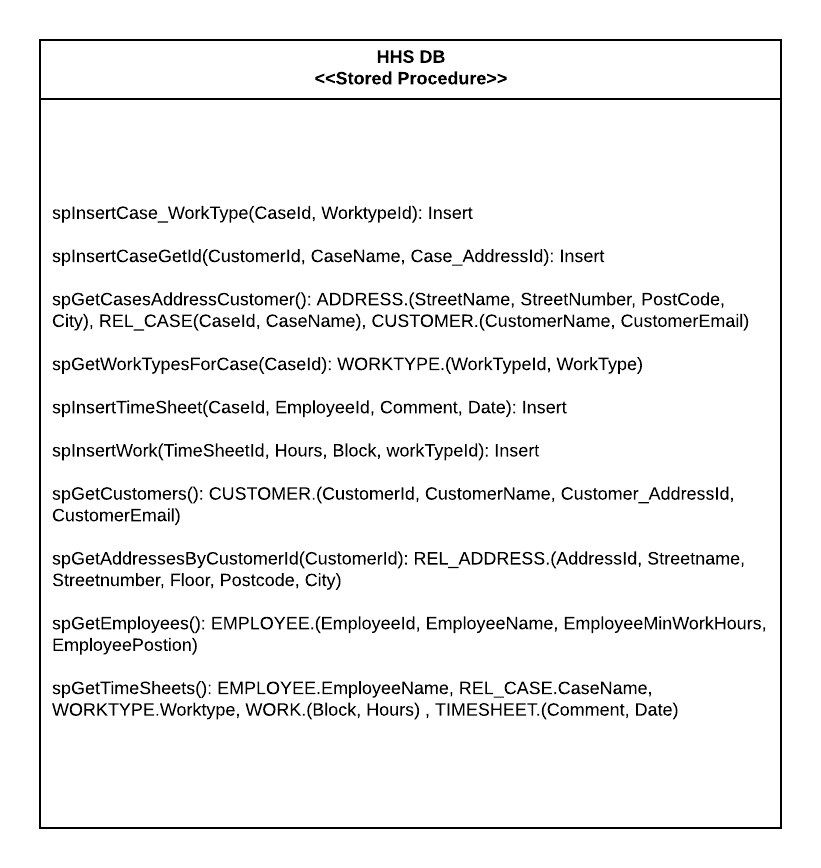
\includegraphics[scale = .7]{DBSP.PNG}}
    \caption{viser de stored procedures, som bliver brugt i databasen, som kan ses i figur \ref{fig:DatabaseDiagram}}
    \label{fig:SP}
\end{figure}

\subsubsection{spGetCaseAddressCustomer}\label{spaddress}
\begin{figure}[H]
    \makebox[\textwidth][c]{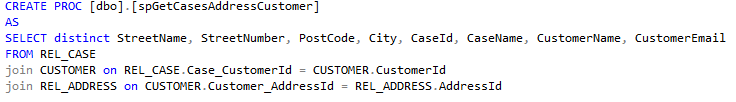
\includegraphics[scale = .6]{SPGETCUSTOMERADDRESS.PNG}}
    \caption{Viser et eksempel på en stored procedure, som henter fra tre forskellige tabeller}
    \label{fig:SPADRRESCUSTOMER}
\end{figure}

I figur \ref{fig:SPADRRESCUSTOMER} ses hvordan proceduren bliver lavet med sproget SQL. Det første der bliver gjort er at bruge SQL kommandoen CREATE PROC, som laver en ny stored procedure, dette er efter fulgt med det navn den skal have.
På linjen under er AS kommandoen, den gør at alt det kode der bliver skrevet efter dette bliver en del af proceduren.
SELECT er den kommando man bruger, når man vil vælge hvilke rækker man gerne vil se.
Der er også blevet valgt, at den skal være distinct, som gør, at der ikke kommer nogle kopier af de forskellige outputs fra rækkerne.
Til sidst specificeres hvor disse rækker skal hentes fra.
Til dette bruges kommandoen FROM.
For at vide, hvor det skal hentes fra bruger vi kommadoerne join og on.
Join bruges, når man gerne vil ligge to tabeller sammen til en samlet tabel.
On bliver altid brugt sammen med join da den bestemmer på hvilke parameter tabellerne skal ligges sammen på.
Join/on bruges hyppigst på at sammenligne primary keys(PK) med foreign keys(FK), som kan ses i figur \ref{fig:DatabaseDiagram}.

\subsubsection{spGetWorkTypesForCase}
\begin{figure}[H]
    \makebox[\textwidth][c]{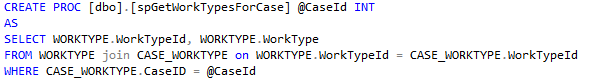
\includegraphics[scale = .7]{SPGETWORKTYPE.PNG}}
    \caption{Viser en stored procedure, der tager en parameter ind som input og bruger denne paramter til at finde et output}
    \label{fig:SPWORKTYPE}
\end{figure}

Stored proceduren i figur \ref{fig:SPWORKTYPE} tager samme udgangspunkt som den anden procedure, forklaret i afsnit \ref{spaddress}.

Forskellen er, at denne stored procedure tager en parameter ind som input.
Denne parameter bliver specificeret oppe ved siden af navnet på proceduren, hvor parameterens navn står, som standard med et \@ tegn foran, og hvilken type den er.
Når der er valgt, hvad der skal bruges med SELECT, og hvor det er fra med FROM, bliver der til sidste specificert præcis den række vi gerne vil have med kommandoen WHERE.
Her siger vi, at caseId skal være den samme, som parameteren.

